\begingroup
\def\imgwidth{5.5cm}

\section{位相シフタコイルによる干渉}
本実験である位相シフタコイルによる干渉について、実験手順、結果、解析の順に説明する。

\subsection{実験手順}
位相シフタコイルに流す電流を、0.0Aから3.3A, -0.3から-1.5までそれぞれ0.3A刻みで変え、各点10分程度測定した。

\subsection{実験結果}
干渉を見るためには、中性子のTOF(波長)を制限する必要がある。
どの波長を選ぶべきか判断するために、様々な波長での実験か結果をフィットして、最もビジビリティが高かった波長を採用することにする。

\paragraph{ビジビリティが最高となる波長}
上流フリッパーと下流フリッパーの反転率が1/2となるのは、予備実験からそれぞれ3.75Å, 3.56Åである。
その付近のいくつかの波長領域について、横軸を位相シフタに流した電流、縦軸をカウント数/LiMのカウント数で割ったものとしてプロットする。
実線は$-A\cos(Bx+C)+D$でフィットした結果を示している。
\begin{figure}[H]
\centering
\begin{minipage}{0.33\hsize}
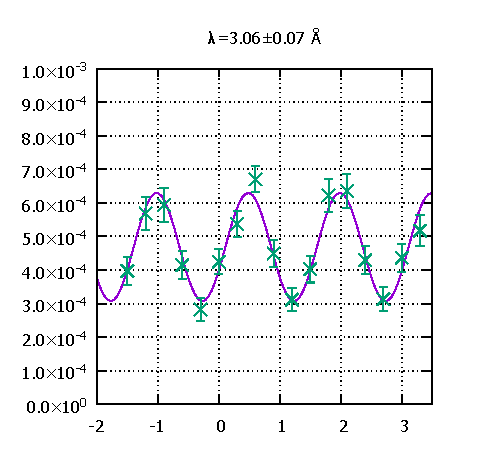
\includegraphics[width=\imgwidth]{phase_shifter/wl/wlf1.pdf}
\end{minipage}
\begin{minipage}{0.33\hsize}
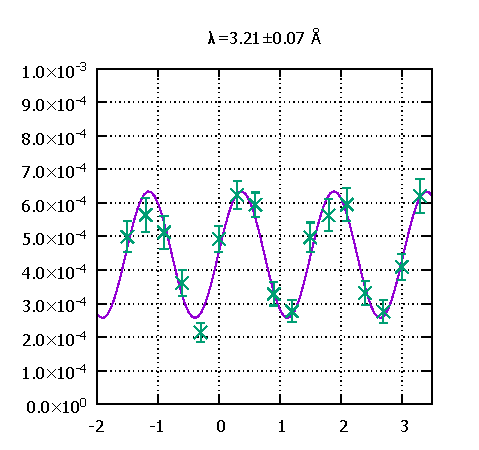
\includegraphics[width=\imgwidth]{phase_shifter/wl/wlf2.pdf}
\end{minipage}
\begin{minipage}{0.33\hsize}
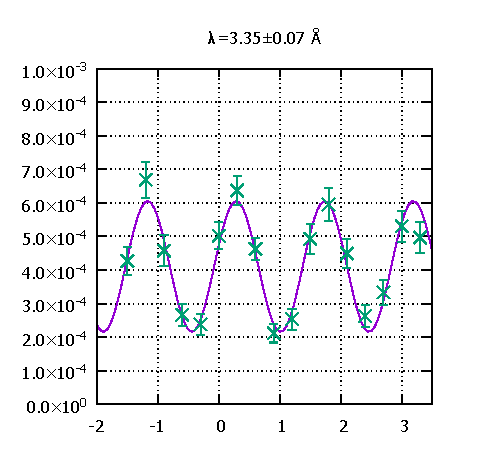
\includegraphics[width=\imgwidth]{phase_shifter/wl/wlf3.pdf}
\end{minipage}\\
\begin{minipage}{0.33\hsize}
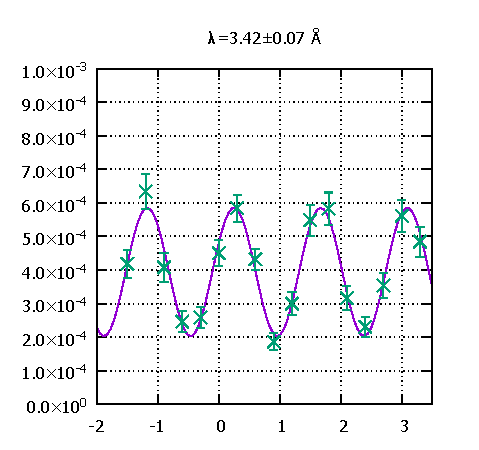
\includegraphics[width=\imgwidth]{phase_shifter/wl/wlf12.pdf}
\end{minipage}
\begin{minipage}{0.33\hsize}
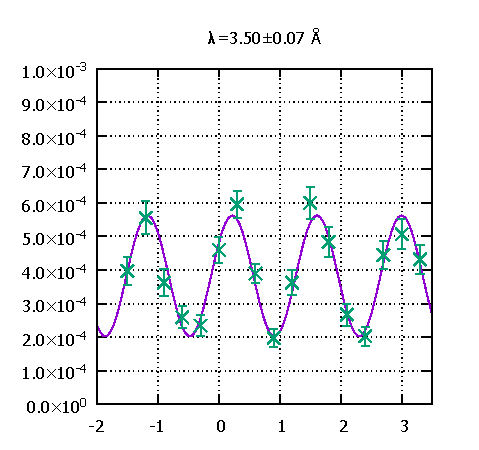
\includegraphics[width=\imgwidth]{phase_shifter/wl/wlf4.pdf}
\end{minipage}
\begin{minipage}{0.33\hsize}
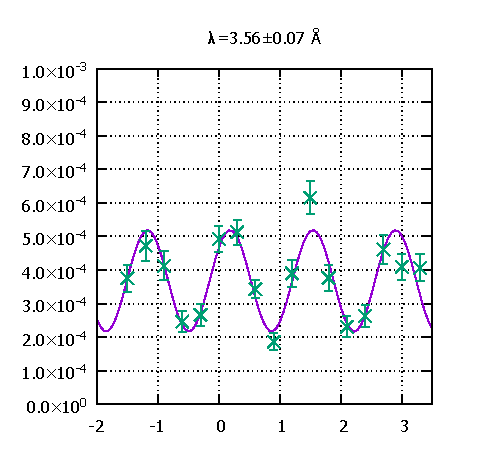
\includegraphics[width=\imgwidth]{phase_shifter/wl/wlf5.pdf}
\end{minipage}
\begin{minipage}{0.33\hsize}
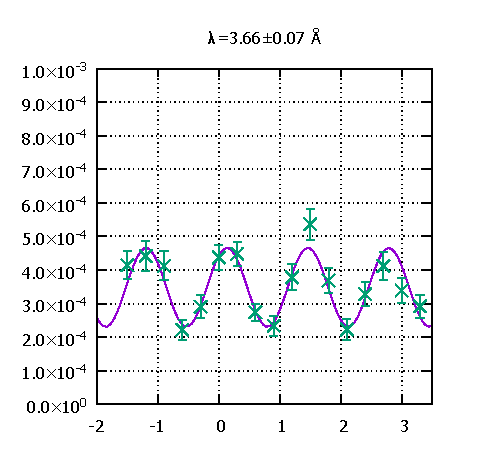
\includegraphics[width=\imgwidth]{phase_shifter/wl/wlf11.pdf}
\end{minipage}
\begin{minipage}{0.33\hsize}
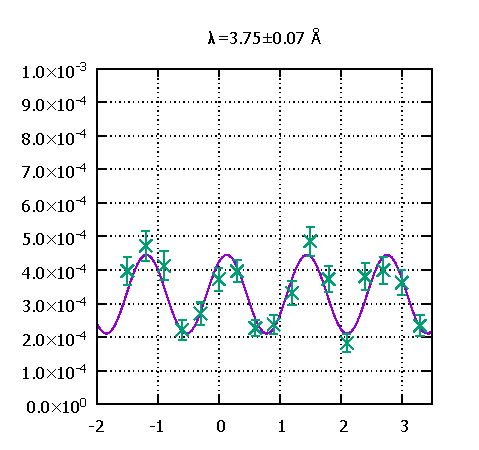
\includegraphics[width=\imgwidth]{phase_shifter/wl/wlf6.pdf}
\end{minipage}
\begin{minipage}{0.33\hsize}
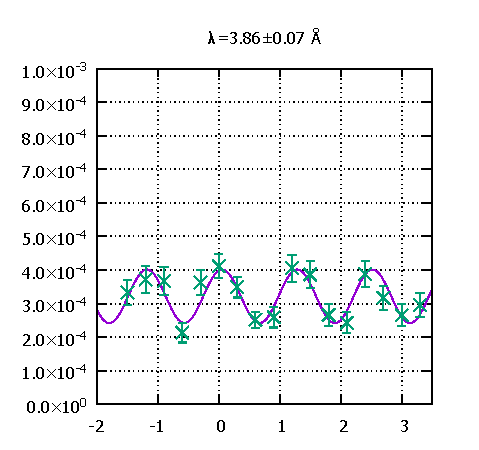
\includegraphics[width=\imgwidth]{phase_shifter/wl/wlf7.pdf}
\end{minipage}
\begin{minipage}{0.33\hsize}
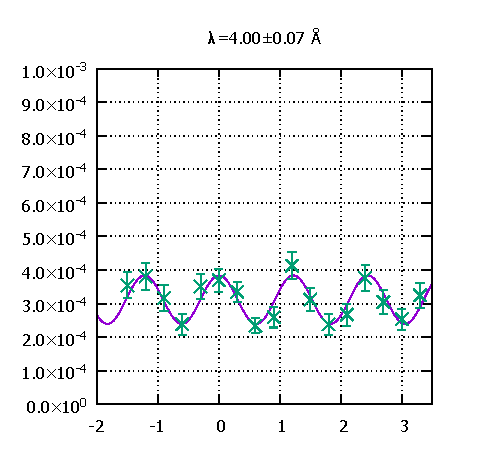
\includegraphics[width=\imgwidth]{phase_shifter/wl/wlf9.pdf}
\end{minipage}
\begin{minipage}{0.33\hsize}
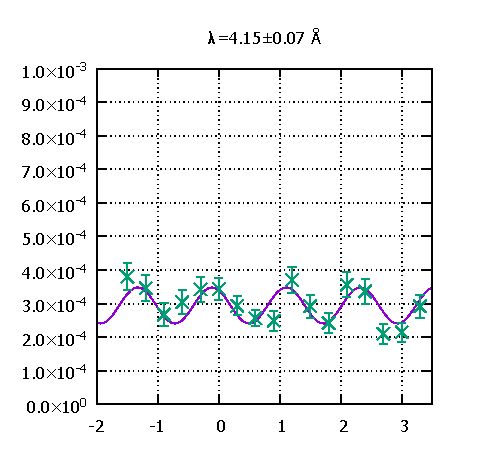
\includegraphics[width=\imgwidth]{phase_shifter/wl/wlf10.pdf}
\end{minipage}
\begin{minipage}{0.33\hsize}
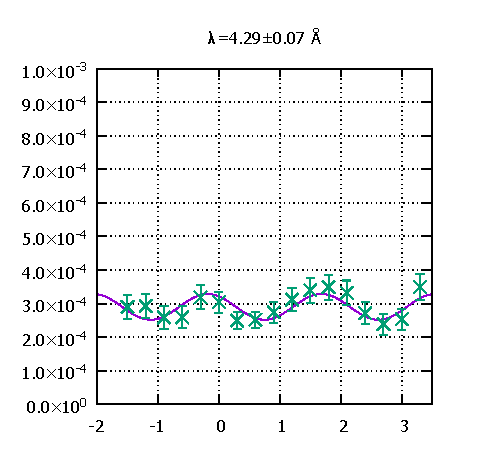
\includegraphics[width=\imgwidth]{phase_shifter/wl/wlf8.pdf}
\end{minipage}
\caption{各波長領域におけるカウント数/LiMカウント数。横軸は位相シフタコイルに流した電流。}
\end{figure}

フィット結果からビジビリティ$V\equiv A/D$を算出し、プロットすると以下のようになる:
\begin{figure}[H]
\centering
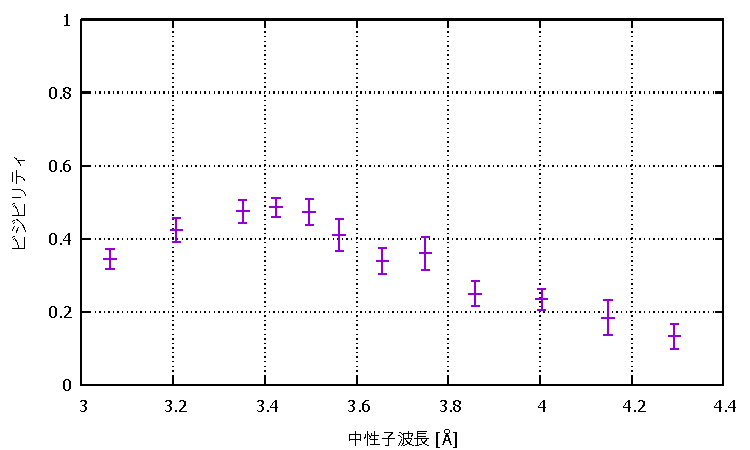
\includegraphics{phase_shifter/visibility.pdf}
\caption{波長ごとのビジビリティ。誤差はフィッティング誤差に由来する。}
\end{figure}

$\lambda=3.42\pm0.07$Åで最もビジビリティが高くなっていることがわかる。

\paragraph{最高ビジビリティとなる波長における結果}
$\lambda=3.42\pm0.07$Åにおける実験結果を以下に示す。
今後の解析はこの波長で行うことにする。
\begin{figure}[H]
\centering
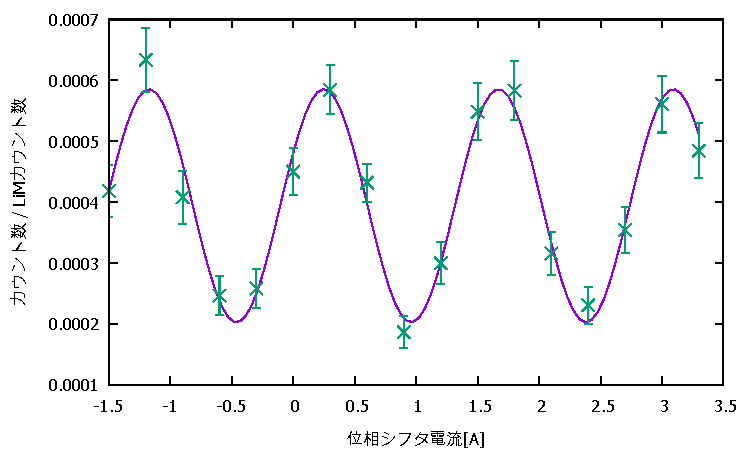
\includegraphics{phase_shifter/fit.pdf}
\caption{$\lambda=3.42\pm0.07$Åにおける実験結果とフィット。\label{ps_fitresult}}
\end{figure}

\subsection{解析}
\paragraph{理論値との対応}
図\ref{ps_fitresult}の縦軸はカウント数/LiMカウント数であり、これは理論値と直接対応する値ではない。
これを理論値と対応付けるために、$|\langle\uparrow|\uparrow\rangle|^2$に対応する、フリッパーをオフにしてスピンをフリップさせずに検出
した時のカウント数/LiMカウント数で割る必要がある。

$\lambda=3.42\pm0.07$Åにおける$|\langle\uparrow|\uparrow\rangle|^2$に対応するカウント数/LiMカウント数は、
$(6.73\pm0.53)\times10^{-4}$であった。この値で規格化した実験結果とフィット結果は以下の通りである:
\begin{figure}[H]
\centering
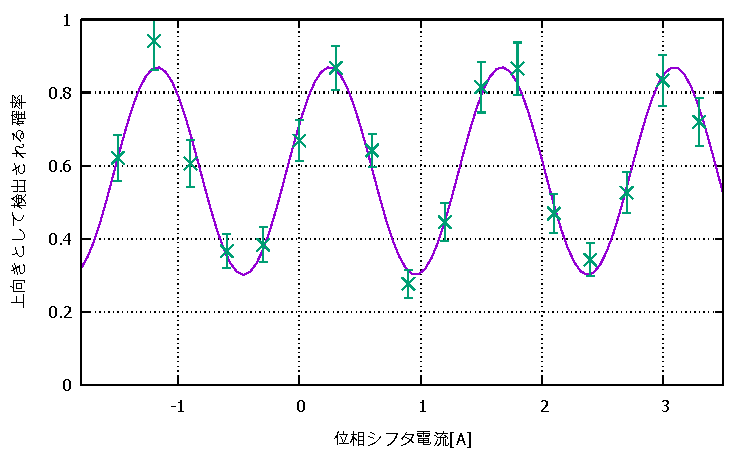
\includegraphics{phase_shifter/highest.pdf}
\end{figure}
\begin{table}[H]
\centering
\begin{tabular}{|r|r|}
\hline
$A$&$0.28\pm0.03$\\
\hline
$B$&$4.42\pm$0.04\\
\hline
$C$&$2.04\pm0.06$\\
\hline
$D$&$0.585\pm0.04$\\
\hline
\end{tabular}
\caption{フィット結果。フィット関数は$-A\cos(Bx+C)+D$}
\end{table}

\paragraph{理論値との比較}
理論式(\ref{theoretical})との比較を行う。
理論式
\begin{align}
|({\psi}_{Ⅶ}(x,t))_{+}|^2
=1-\cos^2\left({\omega}d'/v\right)\sin^2\left(\frac{2\omega_{r}}{v}d\right)\tag{\ref{theoretical}}
\end{align}
のうち、$\sin^2(2\omega_{r}/vd)$については、今$\pi/2$フリップ条件を満たしていることを仮定すれば1である。
従って、以下のように簡略化することができる:
\begin{align}
|({\psi}_{Ⅶ}(x,t))_{+}|^2=\frac{1}{2}\left(
1-\cos\frac{2{\omega}d'}{v}
\right)
\end{align}

$\omega$を電流に対応させることで、理論式の$B$は$4.34$となる。
以上より、理論式のパラメーターをまとめると以下のようになる:
\begin{table}[H]
\centering
\begin{tabular}{|r|r|}
\hline
$A$&$0.5$\\
\hline
$B$&$4.34$\\
\hline
$C$&$0$\\
\hline
$D$&$0.5$\\
\hline
\end{tabular}
\caption{フィット結果。フィット関数は$-A\cos(Bx+C)+D$}
\end{table}

角振動数$B$については$2\sigma$の精度で一致していることがわかる。振幅$A$、位相$C$、オフセット$D$にはずれが見られる。
すれの原因については、後により深く考察する。

\endgroup